\PassOptionsToPackage{unicode=true}{hyperref} % options for packages loaded elsewhere
\PassOptionsToPackage{hyphens}{url}
%
\documentclass[]{article}
\usepackage{lmodern}
\usepackage{amssymb,amsmath}
\usepackage{ifxetex,ifluatex}
\usepackage{fixltx2e} % provides \textsubscript
\ifnum 0\ifxetex 1\fi\ifluatex 1\fi=0 % if pdftex
  \usepackage[T1]{fontenc}
  \usepackage[utf8]{inputenc}
  \usepackage{textcomp} % provides euro and other symbols
\else % if luatex or xelatex
  \usepackage{unicode-math}
  \defaultfontfeatures{Ligatures=TeX,Scale=MatchLowercase}
\fi
% use upquote if available, for straight quotes in verbatim environments
\IfFileExists{upquote.sty}{\usepackage{upquote}}{}
% use microtype if available
\IfFileExists{microtype.sty}{%
\usepackage[]{microtype}
\UseMicrotypeSet[protrusion]{basicmath} % disable protrusion for tt fonts
}{}
\IfFileExists{parskip.sty}{%
\usepackage{parskip}
}{% else
\setlength{\parindent}{0pt}
\setlength{\parskip}{6pt plus 2pt minus 1pt}
}
\usepackage{hyperref}
\hypersetup{
            pdftitle={Wuhan-Hu-1 predictor},
            pdfauthor={Sayantan Ghosh},
            pdfborder={0 0 0},
            breaklinks=true}
\urlstyle{same}  % don't use monospace font for urls
\usepackage[margin=1in]{geometry}
\usepackage{color}
\usepackage{fancyvrb}
\newcommand{\VerbBar}{|}
\newcommand{\VERB}{\Verb[commandchars=\\\{\}]}
\DefineVerbatimEnvironment{Highlighting}{Verbatim}{commandchars=\\\{\}}
% Add ',fontsize=\small' for more characters per line
\usepackage{framed}
\definecolor{shadecolor}{RGB}{248,248,248}
\newenvironment{Shaded}{\begin{snugshade}}{\end{snugshade}}
\newcommand{\AlertTok}[1]{\textcolor[rgb]{0.94,0.16,0.16}{#1}}
\newcommand{\AnnotationTok}[1]{\textcolor[rgb]{0.56,0.35,0.01}{\textbf{\textit{#1}}}}
\newcommand{\AttributeTok}[1]{\textcolor[rgb]{0.77,0.63,0.00}{#1}}
\newcommand{\BaseNTok}[1]{\textcolor[rgb]{0.00,0.00,0.81}{#1}}
\newcommand{\BuiltInTok}[1]{#1}
\newcommand{\CharTok}[1]{\textcolor[rgb]{0.31,0.60,0.02}{#1}}
\newcommand{\CommentTok}[1]{\textcolor[rgb]{0.56,0.35,0.01}{\textit{#1}}}
\newcommand{\CommentVarTok}[1]{\textcolor[rgb]{0.56,0.35,0.01}{\textbf{\textit{#1}}}}
\newcommand{\ConstantTok}[1]{\textcolor[rgb]{0.00,0.00,0.00}{#1}}
\newcommand{\ControlFlowTok}[1]{\textcolor[rgb]{0.13,0.29,0.53}{\textbf{#1}}}
\newcommand{\DataTypeTok}[1]{\textcolor[rgb]{0.13,0.29,0.53}{#1}}
\newcommand{\DecValTok}[1]{\textcolor[rgb]{0.00,0.00,0.81}{#1}}
\newcommand{\DocumentationTok}[1]{\textcolor[rgb]{0.56,0.35,0.01}{\textbf{\textit{#1}}}}
\newcommand{\ErrorTok}[1]{\textcolor[rgb]{0.64,0.00,0.00}{\textbf{#1}}}
\newcommand{\ExtensionTok}[1]{#1}
\newcommand{\FloatTok}[1]{\textcolor[rgb]{0.00,0.00,0.81}{#1}}
\newcommand{\FunctionTok}[1]{\textcolor[rgb]{0.00,0.00,0.00}{#1}}
\newcommand{\ImportTok}[1]{#1}
\newcommand{\InformationTok}[1]{\textcolor[rgb]{0.56,0.35,0.01}{\textbf{\textit{#1}}}}
\newcommand{\KeywordTok}[1]{\textcolor[rgb]{0.13,0.29,0.53}{\textbf{#1}}}
\newcommand{\NormalTok}[1]{#1}
\newcommand{\OperatorTok}[1]{\textcolor[rgb]{0.81,0.36,0.00}{\textbf{#1}}}
\newcommand{\OtherTok}[1]{\textcolor[rgb]{0.56,0.35,0.01}{#1}}
\newcommand{\PreprocessorTok}[1]{\textcolor[rgb]{0.56,0.35,0.01}{\textit{#1}}}
\newcommand{\RegionMarkerTok}[1]{#1}
\newcommand{\SpecialCharTok}[1]{\textcolor[rgb]{0.00,0.00,0.00}{#1}}
\newcommand{\SpecialStringTok}[1]{\textcolor[rgb]{0.31,0.60,0.02}{#1}}
\newcommand{\StringTok}[1]{\textcolor[rgb]{0.31,0.60,0.02}{#1}}
\newcommand{\VariableTok}[1]{\textcolor[rgb]{0.00,0.00,0.00}{#1}}
\newcommand{\VerbatimStringTok}[1]{\textcolor[rgb]{0.31,0.60,0.02}{#1}}
\newcommand{\WarningTok}[1]{\textcolor[rgb]{0.56,0.35,0.01}{\textbf{\textit{#1}}}}
\usepackage{graphicx,grffile}
\makeatletter
\def\maxwidth{\ifdim\Gin@nat@width>\linewidth\linewidth\else\Gin@nat@width\fi}
\def\maxheight{\ifdim\Gin@nat@height>\textheight\textheight\else\Gin@nat@height\fi}
\makeatother
% Scale images if necessary, so that they will not overflow the page
% margins by default, and it is still possible to overwrite the defaults
% using explicit options in \includegraphics[width, height, ...]{}
\setkeys{Gin}{width=\maxwidth,height=\maxheight,keepaspectratio}
\setlength{\emergencystretch}{3em}  % prevent overfull lines
\providecommand{\tightlist}{%
  \setlength{\itemsep}{0pt}\setlength{\parskip}{0pt}}
\setcounter{secnumdepth}{5}
% Redefines (sub)paragraphs to behave more like sections
\ifx\paragraph\undefined\else
\let\oldparagraph\paragraph
\renewcommand{\paragraph}[1]{\oldparagraph{#1}\mbox{}}
\fi
\ifx\subparagraph\undefined\else
\let\oldsubparagraph\subparagraph
\renewcommand{\subparagraph}[1]{\oldsubparagraph{#1}\mbox{}}
\fi

% set default figure placement to htbp
\makeatletter
\def\fps@figure{htbp}
\makeatother


\title{Wuhan-Hu-1 predictor}
\author{Sayantan Ghosh}
\date{2020/12/31}

\begin{document}
\maketitle

{
\setcounter{tocdepth}{2}
\tableofcontents
}
\hypertarget{introduction}{%
\section{Introduction:}\label{introduction}}

The goal of our Covid Project is to show that the poor countries i.e
countries with low per capita income is seen to be not affected by Covid
unlike the rich countries i.e the countries which have a higher per
capita income facing worse effects of Covid.

Function to read the raw CSV files. The files are aggregated to the
country level and then converted to long format.

\begin{Shaded}
\begin{Highlighting}[]
\NormalTok{clean_jhd_to_long <-}\StringTok{ }\ControlFlowTok{function}\NormalTok{(df) \{}
\NormalTok{  df_str <-}\StringTok{ }\KeywordTok{deparse}\NormalTok{(}\KeywordTok{substitute}\NormalTok{(df))}
\NormalTok{  var_str <-}\StringTok{ }\KeywordTok{substr}\NormalTok{(df_str, }\DecValTok{1}\NormalTok{, }\KeywordTok{str_length}\NormalTok{(df_str) }\OperatorTok{-}\StringTok{ }\DecValTok{4}\NormalTok{)}
  
\NormalTok{  df }\OperatorTok\StringTok{ }\KeywordTok{group_by}\NormalTok{(}\StringTok{`}\DataTypeTok{Country/Region}\StringTok{`}\NormalTok{) }\OperatorTok
\StringTok{    }\KeywordTok{filter}\NormalTok{(}\StringTok{`}\DataTypeTok{Country/Region}\StringTok{`} \OperatorTok{!=}\StringTok{ "Cruise Ship"}\NormalTok{) }\OperatorTok
\StringTok{    }\KeywordTok{select}\NormalTok{(}\OperatorTok{-}\StringTok{`}\DataTypeTok{Province/State}\StringTok{`}\NormalTok{, }\OperatorTok{-}\NormalTok{Lat, }\OperatorTok{-}\NormalTok{Long) }\OperatorTok
\StringTok{    }\KeywordTok{mutate_at}\NormalTok{(}\KeywordTok{vars}\NormalTok{(}\OperatorTok{-}\KeywordTok{group_cols}\NormalTok{()), sum) }\OperatorTok\StringTok{ }
\StringTok{    }\KeywordTok{distinct}\NormalTok{() }\OperatorTok
\StringTok{    }\KeywordTok{ungroup}\NormalTok{() }\OperatorTok
\StringTok{    }\KeywordTok{rename}\NormalTok{(}\DataTypeTok{country =} \StringTok{`}\DataTypeTok{Country/Region}\StringTok{`}\NormalTok{) }\OperatorTok
\StringTok{    }\KeywordTok{pivot_longer}\NormalTok{(}
      \OperatorTok{-}\NormalTok{country, }
      \DataTypeTok{names_to =} \StringTok{"date_str"}\NormalTok{, }
      \DataTypeTok{values_to =}\NormalTok{ var_str}
\NormalTok{    ) }\OperatorTok
\StringTok{    }\KeywordTok{mutate}\NormalTok{(}\DataTypeTok{date =} \KeywordTok{mdy}\NormalTok{(date_str)) }\OperatorTok
\StringTok{    }\KeywordTok{select}\NormalTok{(country, date, }\OperatorTok{!!}\StringTok{ }\KeywordTok{sym}\NormalTok{(var_str)) }
\NormalTok{\}}
\end{Highlighting}
\end{Shaded}

\hypertarget{cssegisanddata}{%
\section{CSSEGISandData}\label{cssegisanddata}}

Download datasets

\begin{Shaded}
\begin{Highlighting}[]
\NormalTok{confirmed_raw <-}\StringTok{ }\KeywordTok{read_csv}\NormalTok{(}\StringTok{"https://raw.githubusercontent.com/CSSEGISandData/COVID-19/master/csse_covid_19_data/csse_covid_19_time_series/time_series_covid19_confirmed_global.csv"}\NormalTok{)}
\end{Highlighting}
\end{Shaded}

\begin{verbatim}
## 
## -- Column specification --------------------------------------------------------
## cols(
##   .default = col_double(),
##   `Province/State` = col_character(),
##   `Country/Region` = col_character()
## )
## i Use `spec()` for the full column specifications.
\end{verbatim}

\begin{Shaded}
\begin{Highlighting}[]
\NormalTok{deaths_raw <-}\StringTok{ }\KeywordTok{read_csv}\NormalTok{(}\StringTok{"https://raw.githubusercontent.com/CSSEGISandData/COVID-19/master/csse_covid_19_data/csse_covid_19_time_series/time_series_covid19_deaths_global.csv"}\NormalTok{)}
\end{Highlighting}
\end{Shaded}

\begin{verbatim}
## 
## -- Column specification --------------------------------------------------------
## cols(
##   .default = col_double(),
##   `Province/State` = col_character(),
##   `Country/Region` = col_character()
## )
## i Use `spec()` for the full column specifications.
\end{verbatim}

\begin{Shaded}
\begin{Highlighting}[]
\NormalTok{jh_covid19_data <-}\StringTok{ }\KeywordTok{clean_jhd_to_long}\NormalTok{(confirmed_raw) }\OperatorTok
\StringTok{  }\KeywordTok{full_join}\NormalTok{(}\KeywordTok{clean_jhd_to_long}\NormalTok{(deaths_raw))}
\end{Highlighting}
\end{Shaded}

\begin{verbatim}
## Joining, by = c("country", "date")
\end{verbatim}

Next, I pull official country level indicators from the UN Statstics
Division to get country level identifiers. Merging by country name is
messy. I start with a fuzzy matching approach using the \{stringdist\}
package

\begin{Shaded}
\begin{Highlighting}[]
\NormalTok{jhd_countries <-}\StringTok{ }\KeywordTok{tibble}\NormalTok{(}\DataTypeTok{country =} \KeywordTok{unique}\NormalTok{(jh_covid19_data}\OperatorTok{$}\NormalTok{country)) }\OperatorTok\StringTok{ }\KeywordTok{arrange}\NormalTok{(country)}
\NormalTok{ctry_ids <-}\StringTok{ }\KeywordTok{read_html}\NormalTok{(}\StringTok{"https://unstats.un.org/unsd/methodology/m49/"}\NormalTok{) }\OperatorTok
\StringTok{  }\KeywordTok{html_table}\NormalTok{()}
\NormalTok{un_m49 <-}\StringTok{ }\NormalTok{ctry_ids[[}\DecValTok{1}\NormalTok{]]}
\KeywordTok{colnames}\NormalTok{(un_m49) <-}\StringTok{ }\KeywordTok{c}\NormalTok{(}\StringTok{"country"}\NormalTok{, }\StringTok{"un_m49"}\NormalTok{, }\StringTok{"iso3c"}\NormalTok{)}
\CommentTok{# Data merge}
\NormalTok{ctry_names_dist <-}\StringTok{ }\KeywordTok{matrix}\NormalTok{(}\OtherTok{NA}\NormalTok{, }\DataTypeTok{nrow =} \KeywordTok{nrow}\NormalTok{(jhd_countries), }\DataTypeTok{ncol =} \KeywordTok{nrow}\NormalTok{(un_m49))}
\ControlFlowTok{for}\NormalTok{(i }\ControlFlowTok{in} \DecValTok{1}\OperatorTok{:}\KeywordTok{length}\NormalTok{(jhd_countries}\OperatorTok{$}\NormalTok{country)) \{}
  \ControlFlowTok{for}\NormalTok{(j }\ControlFlowTok{in} \DecValTok{1}\OperatorTok{:}\KeywordTok{length}\NormalTok{(un_m49}\OperatorTok{$}\NormalTok{country)) \{ }
\NormalTok{    ctry_names_dist[i,j]<-}\KeywordTok{stringdist}\NormalTok{(}\KeywordTok{tolower}\NormalTok{(jhd_countries}\OperatorTok{$}\NormalTok{country[i]), }
                                     \KeywordTok{tolower}\NormalTok{(un_m49}\OperatorTok{$}\NormalTok{country[j]))      }
\NormalTok{  \}  }
\NormalTok{\}}
\end{Highlighting}
\end{Shaded}

This matches most cases well but some cases need to be adjusted by hand.
In addition there are two jurisdictions (Kosovo, Taiwan) that cannot be
matched as they are no `country' as far as the U.N. Statistics Devision
is concerned.

\hypertarget{watch-out}{%
\section{WATCH OUT:}\label{watch-out}}

\textbf{The data from JHU is subject to change without notice.} New
countries are being added and names/spelling might change.Also, in the
long run, the data provided by the UNSD might change.

\begin{Shaded}
\begin{Highlighting}[]
\NormalTok{min_ctry_name_dist <-}\StringTok{ }\KeywordTok{apply}\NormalTok{(ctry_names_dist, }\DecValTok{1}\NormalTok{, min)}
\NormalTok{matched_ctry_names <-}\StringTok{ }\OtherTok{NULL}
\ControlFlowTok{for}\NormalTok{(i }\ControlFlowTok{in} \DecValTok{1}\OperatorTok{:}\KeywordTok{nrow}\NormalTok{(jhd_countries)) \{}
\NormalTok{  un_m49_row <-}\StringTok{ }\KeywordTok{match}\NormalTok{(min_ctry_name_dist[i], ctry_names_dist[i,])}
  \ControlFlowTok{if}\NormalTok{ (}\KeywordTok{length}\NormalTok{(}\KeywordTok{which}\NormalTok{(ctry_names_dist[i,] }\OperatorTok\StringTok{ }\NormalTok{min_ctry_name_dist[i])) }\OperatorTok{>}\StringTok{ }\DecValTok{1}\NormalTok{) un_m49_row <-}\StringTok{ }\OtherTok{NA}
\NormalTok{  matched_ctry_names <-}\StringTok{ }\KeywordTok{rbind}\NormalTok{(matched_ctry_names,}
                              \KeywordTok{tibble}\NormalTok{( }
                                \DataTypeTok{jhd_countries_row =}\NormalTok{ i, }
                                \DataTypeTok{un_m49_row =}\NormalTok{ un_m49_row,}
                                \DataTypeTok{jhd_ctry_name =}\NormalTok{ jhd_countries}\OperatorTok{$}\NormalTok{country[i], }
                                \DataTypeTok{un_m49_name =} \KeywordTok{ifelse}\NormalTok{(}\KeywordTok{is.na}\NormalTok{(un_m49_row), }\OtherTok{NA}\NormalTok{, }
\NormalTok{                                                     un_m49}\OperatorTok{$}\NormalTok{country[un_m49_row])}
\NormalTok{                              ))}
\NormalTok{\}}
\CommentTok{# Inspect 'matched_ctry_names' before using the data.}
\NormalTok{matched_ctry_names}\OperatorTok{$}\NormalTok{un_m49_row[matched_ctry_names}\OperatorTok{$}\NormalTok{jhd_ctry_name }\OperatorTok{==}\StringTok{ "Bolivia"}\NormalTok{] <-}\StringTok{ }\DecValTok{27}
\NormalTok{matched_ctry_names}\OperatorTok{$}\NormalTok{un_m49_row[matched_ctry_names}\OperatorTok{$}\NormalTok{jhd_ctry_name }\OperatorTok{==}\StringTok{ "Brunei"}\NormalTok{] <-}\StringTok{ }\DecValTok{35}
\NormalTok{matched_ctry_names}\OperatorTok{$}\NormalTok{un_m49_row[matched_ctry_names}\OperatorTok{$}\NormalTok{jhd_ctry_name }\OperatorTok{==}\StringTok{ "Congo (Brazzaville)"}\NormalTok{] <-}\StringTok{ }\DecValTok{54}
\NormalTok{matched_ctry_names}\OperatorTok{$}\NormalTok{un_m49_row[matched_ctry_names}\OperatorTok{$}\NormalTok{jhd_ctry_name }\OperatorTok{==}\StringTok{ "Congo (Kinshasa)"}\NormalTok{] <-}\StringTok{ }\DecValTok{64}
\NormalTok{matched_ctry_names}\OperatorTok{$}\NormalTok{un_m49_row[matched_ctry_names}\OperatorTok{$}\NormalTok{jhd_ctry_name }\OperatorTok{==}\StringTok{ "East Timor"}\NormalTok{] <-}\StringTok{ }\DecValTok{222}
\NormalTok{matched_ctry_names}\OperatorTok{$}\NormalTok{un_m49_row[matched_ctry_names}\OperatorTok{$}\NormalTok{jhd_ctry_name }\OperatorTok{==}\StringTok{ "Iran"}\NormalTok{] <-}\StringTok{ }\DecValTok{109}
\NormalTok{matched_ctry_names}\OperatorTok{$}\NormalTok{un_m49_row[matched_ctry_names}\OperatorTok{$}\NormalTok{jhd_ctry_name }\OperatorTok{==}\StringTok{ "Korea, South"}\NormalTok{] <-}\StringTok{ }\DecValTok{180}
\NormalTok{matched_ctry_names}\OperatorTok{$}\NormalTok{un_m49_row[matched_ctry_names}\OperatorTok{$}\NormalTok{jhd_ctry_name }\OperatorTok{==}\StringTok{ "Kosovo"}\NormalTok{] <-}\StringTok{ }\OtherTok{NA}
\NormalTok{matched_ctry_names}\OperatorTok{$}\NormalTok{un_m49_row[matched_ctry_names}\OperatorTok{$}\NormalTok{jhd_ctry_name }\OperatorTok{==}\StringTok{ "Moldova"}\NormalTok{] <-}\StringTok{ }\DecValTok{181}
\NormalTok{matched_ctry_names}\OperatorTok{$}\NormalTok{un_m49_row[matched_ctry_names}\OperatorTok{$}\NormalTok{jhd_ctry_name }\OperatorTok{==}\StringTok{ "Russia"}\NormalTok{] <-}\StringTok{ }\DecValTok{184}
\NormalTok{matched_ctry_names}\OperatorTok{$}\NormalTok{un_m49_row[matched_ctry_names}\OperatorTok{$}\NormalTok{jhd_ctry_name }\OperatorTok{==}\StringTok{ "Taiwan*"}\NormalTok{] <-}\StringTok{ }\OtherTok{NA}
\NormalTok{matched_ctry_names}\OperatorTok{$}\NormalTok{un_m49_row[matched_ctry_names}\OperatorTok{$}\NormalTok{jhd_ctry_name }\OperatorTok{==}\StringTok{ "Tanzania"}\NormalTok{] <-}\StringTok{ }\DecValTok{236}
\NormalTok{matched_ctry_names}\OperatorTok{$}\NormalTok{un_m49_row[matched_ctry_names}\OperatorTok{$}\NormalTok{jhd_ctry_name }\OperatorTok{==}\StringTok{ "United Kingdom"}\NormalTok{] <-}\StringTok{ }\DecValTok{235}
\NormalTok{matched_ctry_names}\OperatorTok{$}\NormalTok{un_m49_row[matched_ctry_names}\OperatorTok{$}\NormalTok{jhd_ctry_name }\OperatorTok{==}\StringTok{ "US"}\NormalTok{] <-}\StringTok{ }\DecValTok{238}
\NormalTok{matched_ctry_names}\OperatorTok{$}\NormalTok{un_m49_row[matched_ctry_names}\OperatorTok{$}\NormalTok{jhd_ctry_name }\OperatorTok{==}\StringTok{ "Venezuela"}\NormalTok{] <-}\StringTok{ }\DecValTok{243}
\CommentTok{# Last Step: Match country identifier data }
\NormalTok{jhd_countries }\OperatorTok\StringTok{ }
\StringTok{  }\KeywordTok{left_join}\NormalTok{(matched_ctry_names }\OperatorTok\StringTok{ }
\StringTok{              }\KeywordTok{select}\NormalTok{(jhd_ctry_name, un_m49_row), }
            \DataTypeTok{by =} \KeywordTok{c}\NormalTok{(}\DataTypeTok{country =} \StringTok{"jhd_ctry_name"}\NormalTok{)) }\OperatorTok
\StringTok{  }\KeywordTok{left_join}\NormalTok{(un_m49 }\OperatorTok\StringTok{ }\KeywordTok{mutate}\NormalTok{(}\DataTypeTok{un_m49_row =} \KeywordTok{row_number}\NormalTok{()), }\DataTypeTok{by =} \StringTok{"un_m49_row"}\NormalTok{) }\OperatorTok
\StringTok{  }\KeywordTok{rename}\NormalTok{(}\DataTypeTok{country =}\NormalTok{ country.x) }\OperatorTok
\StringTok{  }\KeywordTok{select}\NormalTok{(country, iso3c)  ->}\StringTok{ }\NormalTok{jhd_countries}
\NormalTok{jh_covid19_data <-}\StringTok{ }\NormalTok{jh_covid19_data }\OperatorTok\StringTok{ }\KeywordTok{left_join}\NormalTok{(jhd_countries) }\OperatorTok
\StringTok{  }\KeywordTok{select}\NormalTok{(country, iso3c, date, confirmed, deaths)}
\end{Highlighting}
\end{Shaded}

\begin{verbatim}
## Joining, by = "country"
\end{verbatim}

\begin{Shaded}
\begin{Highlighting}[]
\CommentTok{# we can save the file for future use. not using this approach anymore}
\CommentTok{# write_csv(jh_covid19_data, sprintf("jh_covid19_data_%s.csv", Sys.Date()))}
\end{Highlighting}
\end{Shaded}

\hypertarget{worldbank-data}{%
\section{worldbank data}\label{worldbank-data}}

Merge Covid data with Worldbank data for GDP and population details.
Then convert year format for proper plotting and add other relevant
columns.

\begin{Shaded}
\begin{Highlighting}[]
\NormalTok{pull_worldbank_data <-}\StringTok{ }\ControlFlowTok{function}\NormalTok{(vars) \{}
\NormalTok{  new_cache <-}\StringTok{ }\KeywordTok{wbcache}\NormalTok{()}
\NormalTok{  all_vars <-}\StringTok{ }\KeywordTok{as.character}\NormalTok{(}\KeywordTok{unique}\NormalTok{(new_cache}\OperatorTok{$}\NormalTok{indicators}\OperatorTok{$}\NormalTok{indicatorID))}
\NormalTok{  data_wide <-}\StringTok{ }\KeywordTok{wb}\NormalTok{(}\DataTypeTok{indicator =}\NormalTok{ vars, }\DataTypeTok{mrv =} \DecValTok{10}\NormalTok{, }\DataTypeTok{return_wide =} \OtherTok{TRUE}\NormalTok{)}
\NormalTok{  new_cache}\OperatorTok{$}\NormalTok{indicators[new_cache}\OperatorTok{$}\NormalTok{indicators[,}\StringTok{"indicatorID"}\NormalTok{] }\OperatorTok\StringTok{ }\NormalTok{vars, ] }\OperatorTok
\StringTok{    }\KeywordTok{rename}\NormalTok{(}\DataTypeTok{var_name =}\NormalTok{ indicatorID) }\OperatorTok
\StringTok{    }\KeywordTok{mutate}\NormalTok{(}\DataTypeTok{var_def =} \KeywordTok{paste}\NormalTok{(indicator, }\StringTok{"}\CharTok{\textbackslash{}n}\StringTok{Note:"}\NormalTok{,}
\NormalTok{                           indicatorDesc, }\StringTok{"}\CharTok{\textbackslash{}n}\StringTok{Source:"}\NormalTok{, sourceOrg)) }\OperatorTok
\StringTok{    }\KeywordTok{select}\NormalTok{(var_name, var_def) ->}\StringTok{ }\NormalTok{wb_data_def}
\NormalTok{  new_cache}\OperatorTok{$}\NormalTok{countries }\OperatorTok
\StringTok{    }\KeywordTok{select}\NormalTok{(iso3c, iso2c, country, region, income) ->}\StringTok{ }\NormalTok{ctries}
  \KeywordTok{left_join}\NormalTok{(data_wide, ctries, }\DataTypeTok{by =} \StringTok{"iso3c"}\NormalTok{) }\OperatorTok
\StringTok{    }\KeywordTok{rename}\NormalTok{(}\DataTypeTok{year =}\NormalTok{ date,}
           \DataTypeTok{iso2c =}\NormalTok{ iso2c.y,}
           \DataTypeTok{country =}\NormalTok{ country.y) }\OperatorTok
\StringTok{    }\KeywordTok{select}\NormalTok{(iso3c, iso2c, country, region, income, }\KeywordTok{everything}\NormalTok{()) }\OperatorTok
\StringTok{    }\KeywordTok{select}\NormalTok{(}\OperatorTok{-}\NormalTok{iso2c.x, }\OperatorTok{-}\NormalTok{country.x) }\OperatorTok
\StringTok{    }\KeywordTok{filter}\NormalTok{(}\OperatorTok{!}\KeywordTok{is.na}\NormalTok{(NY.GDP.PCAP.KD),}
\NormalTok{           region }\OperatorTok{!=}\StringTok{ "Aggregates"}\NormalTok{) ->}\StringTok{ }\NormalTok{wb_data}
\NormalTok{  wb_data}\OperatorTok{$}\NormalTok{year <-}\StringTok{ }\KeywordTok{as.numeric}\NormalTok{(wb_data}\OperatorTok{$}\NormalTok{year)}
\NormalTok{  wb_data_def<-}\StringTok{ }\KeywordTok{left_join}\NormalTok{(}\KeywordTok{data.frame}\NormalTok{(}\DataTypeTok{var_name =} \KeywordTok{names}\NormalTok{(wb_data),}
                                     \DataTypeTok{stringsAsFactors =} \OtherTok{FALSE}\NormalTok{),}
\NormalTok{                          wb_data_def, }\DataTypeTok{by =} \StringTok{"var_name"}\NormalTok{)}
\NormalTok{  wb_data_def}\OperatorTok{$}\NormalTok{var_def[}\DecValTok{1}\OperatorTok{:}\DecValTok{6}\NormalTok{] <-}\StringTok{ }\KeywordTok{c}\NormalTok{(}
    \StringTok{"Three letter ISO country code as used by World Bank"}\NormalTok{,}
    \StringTok{"Two letter ISO country code as used by World Bank"}\NormalTok{,}
    \StringTok{"Country name as used by World Bank"}\NormalTok{,}
    \StringTok{"World Bank regional country classification"}\NormalTok{,}
    \StringTok{"World Bank income group classification"}\NormalTok{,}
    \StringTok{"Calendar year of observation"}
\NormalTok{  )}
\NormalTok{  wb_data_def}\OperatorTok{$}\NormalTok{type =}\StringTok{ }\KeywordTok{c}\NormalTok{(}\StringTok{"cs_id"}\NormalTok{, }\KeywordTok{rep}\NormalTok{(}\StringTok{"factor"}\NormalTok{,  }\DecValTok{4}\NormalTok{), }\StringTok{"ts_id"}\NormalTok{,}
                       \KeywordTok{rep}\NormalTok{(}\StringTok{"numeric"}\NormalTok{, }\KeywordTok{ncol}\NormalTok{(wb_data) }\OperatorTok{-}\StringTok{ }\DecValTok{6}\NormalTok{))}
  \KeywordTok{return}\NormalTok{(}\KeywordTok{list}\NormalTok{(wb_data, wb_data_def))}
\NormalTok{\}}
\CommentTok{# define population and locality variables }
\NormalTok{vars <-}\StringTok{ }\KeywordTok{c}\NormalTok{(}\StringTok{"SP.POP.TOTL"}\NormalTok{, }\StringTok{"AG.LND.TOTL.K2"}\NormalTok{, }\StringTok{"EN.POP.DNST"}\NormalTok{, }\StringTok{"EN.URB.LCTY"}\NormalTok{, }\StringTok{"SP.DYN.LE00.IN"}\NormalTok{, }\StringTok{"NY.GDP.PCAP.KD"}\NormalTok{)}
\CommentTok{# then use them in wb_list}
\NormalTok{wb_list <-}\StringTok{ }\KeywordTok{pull_worldbank_data}\NormalTok{(vars)}
\end{Highlighting}
\end{Shaded}

\begin{verbatim}
## Warning: `wbcache()` is deprecated as of wbstats 1.0.0.
## Please use `wb_cache()` instead.
## This warning is displayed once every 8 hours.
## Call `lifecycle::last_warnings()` to see where this warning was generated.
\end{verbatim}

\begin{verbatim}
## Warning: `wb()` is deprecated as of wbstats 1.0.0.
## Please use `wb_data()` instead.
## This warning is displayed once every 8 hours.
## Call `lifecycle::last_warnings()` to see where this warning was generated.
\end{verbatim}

\begin{Shaded}
\begin{Highlighting}[]
\NormalTok{wb_data <-}\StringTok{ }\NormalTok{wb_list[[}\DecValTok{1}\NormalTok{]]}
\NormalTok{wb_data_def <-}\StringTok{ }\NormalTok{wb_list[[}\DecValTok{2}\NormalTok{]]}
\CommentTok{# summarize wordbank data to get country wise details.}
\NormalTok{wb_data }\OperatorTok
\StringTok{  }\KeywordTok{group_by}\NormalTok{(iso3c) }\OperatorTok
\StringTok{  }\KeywordTok{arrange}\NormalTok{(iso3c, year) }\OperatorTok
\StringTok{  }\KeywordTok{summarise}\NormalTok{(}
    \DataTypeTok{population =} \KeywordTok{last}\NormalTok{(}\KeywordTok{na.omit}\NormalTok{(SP.POP.TOTL)),}
    \DataTypeTok{land_area_skm =} \KeywordTok{last}\NormalTok{(}\KeywordTok{na.omit}\NormalTok{(AG.LND.TOTL.K2)),}
    \DataTypeTok{pop_density =} \KeywordTok{last}\NormalTok{(}\KeywordTok{na.omit}\NormalTok{(EN.POP.DNST)),}
    \DataTypeTok{pop_largest_city =} \KeywordTok{last}\NormalTok{(}\KeywordTok{na.omit}\NormalTok{(EN.URB.LCTY)),}
    \DataTypeTok{gdp_capita =} \KeywordTok{last}\NormalTok{(}\KeywordTok{na.omit}\NormalTok{(NY.GDP.PCAP.KD)),}
    \DataTypeTok{life_expectancy =} \KeywordTok{last}\NormalTok{(}\KeywordTok{na.omit}\NormalTok{(SP.DYN.LE00.IN))}
\NormalTok{  ) }\OperatorTok\StringTok{ }\KeywordTok{left_join}\NormalTok{(wb_data }\OperatorTok\StringTok{ }\KeywordTok{select}\NormalTok{(iso3c, region, income) }\OperatorTok\StringTok{ }\KeywordTok{distinct}\NormalTok{()) ->}\StringTok{ }\NormalTok{wb_cs}
\end{Highlighting}
\end{Shaded}

\begin{verbatim}
## `summarise()` has grouped output by 'iso3c'. You can override using the `.groups` argument.
\end{verbatim}

\begin{verbatim}
## Joining, by = "iso3c"
\end{verbatim}

\begin{Shaded}
\begin{Highlighting}[]
\CommentTok{# write_csv(wb_cs, "jh_add_wbank_data.csv")}
\end{Highlighting}
\end{Shaded}

I define event time zero where, for a given country, the confirmed cases
match or exceed the Chinese case number at the beginning of the data so
that all countries can be compared across event time. Also a require
each country to have at least 7 days post event day 0.

\begin{Shaded}
\begin{Highlighting}[]
\NormalTok{dta <-}\StringTok{ }\NormalTok{jh_covid19_data }\OperatorTok\StringTok{ }\KeywordTok{mutate}\NormalTok{(}\DataTypeTok{date =} \KeywordTok{ymd}\NormalTok{(date))}
\CommentTok{# Time event zero}
\NormalTok{dta }\OperatorTok\StringTok{ }
\StringTok{  }\KeywordTok{group_by}\NormalTok{(country) }\OperatorTok
\StringTok{  }\KeywordTok{filter}\NormalTok{(confirmed }\OperatorTok{>=}\StringTok{ }\KeywordTok{min}\NormalTok{(dta}\OperatorTok{$}\NormalTok{confirmed[dta}\OperatorTok{$}\NormalTok{country }\OperatorTok{==}\StringTok{ "China"}\NormalTok{])) }\OperatorTok
\StringTok{  }\KeywordTok{summarise}\NormalTok{(}\DataTypeTok{edate_confirmed =} \KeywordTok{min}\NormalTok{(date)) ->}\StringTok{ }\NormalTok{edates_confirmed}
\CommentTok{# extract significant values and add a column for per hundred thousand population}
\NormalTok{dta }\OperatorTok\StringTok{ }
\StringTok{  }\KeywordTok{left_join}\NormalTok{(edates_confirmed, }\DataTypeTok{by =} \StringTok{"country"}\NormalTok{) }\OperatorTok
\StringTok{  }\KeywordTok{mutate}\NormalTok{(}
    \DataTypeTok{edate_confirmed =} \KeywordTok{as.numeric}\NormalTok{(date }\OperatorTok{-}\StringTok{ }\NormalTok{edate_confirmed)}
\NormalTok{  ) }\OperatorTok
\StringTok{  }\KeywordTok{filter}\NormalTok{(edate_confirmed }\OperatorTok{>=}\StringTok{ }\DecValTok{0}\NormalTok{) }\OperatorTok
\StringTok{  }\KeywordTok{group_by}\NormalTok{(country) }\OperatorTok
\StringTok{  }\KeywordTok{filter}\NormalTok{ (}\KeywordTok{n}\NormalTok{() }\OperatorTok{>=}\StringTok{ }\DecValTok{7}\NormalTok{) }\OperatorTok\StringTok{ }
\StringTok{  }\KeywordTok{ungroup}\NormalTok{() }\OperatorTok
\StringTok{  }\KeywordTok{left_join}\NormalTok{(wb_cs, }\DataTypeTok{by =} \StringTok{"iso3c"}\NormalTok{) }\OperatorTok\StringTok{ }
\StringTok{  }\KeywordTok{mutate}\NormalTok{(}
    \DataTypeTok{confirmed_1e5pop =} \FloatTok{1e5}\OperatorTok{*}\NormalTok{confirmed}\OperatorTok{/}\NormalTok{population}
\NormalTok{  ) ->}\StringTok{ }\NormalTok{df}
\end{Highlighting}
\end{Shaded}

Data as provided by Johns Hopkins University Center for Systems Science
and Engineering (JHU CSSE) The sample is limited to countries with at
least seven days of positive event days data.

\begin{Shaded}
\begin{Highlighting}[]
\NormalTok{lab_notes <-}\StringTok{ }\KeywordTok{paste0}\NormalTok{(}
  \StringTok{"Data as provided by Johns Hopkins University Center for Systems Science "}\NormalTok{, }
  \StringTok{"and Engineering (JHU CSSE)}\CharTok{\textbackslash{}n}\StringTok{and obtained on March 23, 2020. "}\NormalTok{,}
  \StringTok{"The sample is limited to countries with at least seven days of positive}\CharTok{\textbackslash{}n}\StringTok{"}\NormalTok{, }
  \StringTok{"event days data."}
\NormalTok{)}
\NormalTok{lab_x_axis_confirmed <-}\StringTok{ }\KeywordTok{sprintf}\NormalTok{(}\KeywordTok{paste}\NormalTok{(}
  \StringTok{"Days since confirmed cases matched or exceeded}\CharTok{\textbackslash{}n}\StringTok{"}\NormalTok{, }
  \StringTok{"initial value reported for China (%d cases)}\CharTok{\textbackslash{}n}\StringTok{"}
\NormalTok{), }\KeywordTok{min}\NormalTok{(dta}\OperatorTok{$}\NormalTok{confirmed[dta}\OperatorTok{$}\NormalTok{country }\OperatorTok{==}\StringTok{ "China"}\NormalTok{]))}
\NormalTok{gg_my_blob <-}\StringTok{ }\KeywordTok{list}\NormalTok{(}
  \KeywordTok{scale_y_continuous}\NormalTok{(}\DataTypeTok{trans=}\StringTok{'log10'}\NormalTok{, }\DataTypeTok{labels =}\NormalTok{ scales}\OperatorTok{::}\NormalTok{comma),  }
  \KeywordTok{theme_minimal}\NormalTok{(), }
  \KeywordTok{theme}\NormalTok{(}
    \CommentTok{#plot.title.position = "plot", }
    \CommentTok{#plot.caption.position =  "plot",}
    \DataTypeTok{plot.caption =} \KeywordTok{element_text}\NormalTok{(}\DataTypeTok{hjust =} \DecValTok{0}\NormalTok{),}
    \DataTypeTok{axis.title.x =} \KeywordTok{element_text}\NormalTok{(}\DataTypeTok{hjust =} \DecValTok{1}\NormalTok{),}
    \DataTypeTok{axis.title.y =} \KeywordTok{element_text}\NormalTok{(}\DataTypeTok{hjust =} \DecValTok{1}\NormalTok{),}
\NormalTok{  ),}
  \KeywordTok{labs}\NormalTok{(}\DataTypeTok{caption =}\NormalTok{ lab_notes,}
       \DataTypeTok{x =}\NormalTok{ lab_x_axis_confirmed,}
       \DataTypeTok{y =} \StringTok{"Confirmed cases (logarithmic scale)"}\NormalTok{),}
  \KeywordTok{gghighlight}\NormalTok{(}\OtherTok{TRUE}\NormalTok{,  }\DataTypeTok{label_key =}\NormalTok{ country, }\DataTypeTok{use_direct_label =} \OtherTok{TRUE}\NormalTok{,}
              \DataTypeTok{label_params =} \KeywordTok{list}\NormalTok{(}\DataTypeTok{segment.color =} \OtherTok{NA}\NormalTok{, }\DataTypeTok{nudge_x =} \DecValTok{1}\NormalTok{))}
\NormalTok{)}
\end{Highlighting}
\end{Shaded}

The base plot confirmed cases per 100,000 inhabitants generated for a
representative sample of countries.

\begin{Shaded}
\begin{Highlighting}[]
\KeywordTok{ggplot}\NormalTok{(df }\OperatorTok\StringTok{ }\KeywordTok{filter}\NormalTok{ (country }\OperatorTok{==}\StringTok{ }\KeywordTok{c}\NormalTok{(}\StringTok{"US"}\NormalTok{,}\StringTok{"United Kingdom"}\NormalTok{,}\StringTok{"New Zealand"}\NormalTok{,}\StringTok{"India"}\NormalTok{,}\StringTok{"Ghana"}\NormalTok{,}\StringTok{"Zambia"}\NormalTok{,}\StringTok{"Zimbabwe"}\NormalTok{)), }
       \KeywordTok{aes}\NormalTok{(}\DataTypeTok{x =}\NormalTok{ edate_confirmed, }\DataTypeTok{color =}\NormalTok{ country, }\DataTypeTok{y =}\NormalTok{ confirmed_}\FloatTok{1e5}\NormalTok{pop)) }\OperatorTok{+}
\StringTok{  }\KeywordTok{geom_line}\NormalTok{() }\OperatorTok{+}
\StringTok{  }\NormalTok{gg_my_blob }\OperatorTok{+}
\StringTok{  }\KeywordTok{labs}\NormalTok{(}
    \DataTypeTok{y =} \StringTok{"Confirmed cases per 100,000 inhabitants"}\NormalTok{,}
    \DataTypeTok{title =} \StringTok{"Cases relative to population}\CharTok{\textbackslash{}n}\StringTok{"}
\NormalTok{  ) }
\end{Highlighting}
\end{Shaded}

\begin{verbatim}
## Warning in country == c("US", "United Kingdom", "New Zealand", "India", : longer
## object length is not a multiple of shorter object length
\end{verbatim}

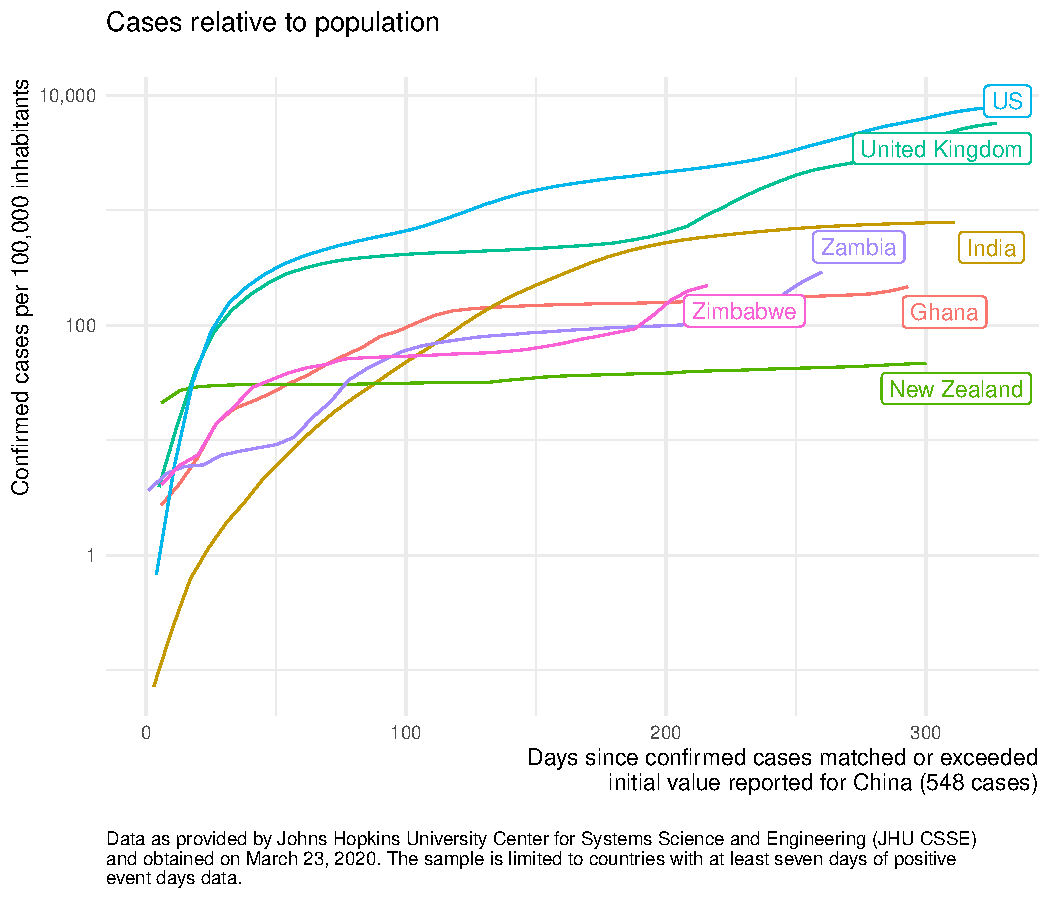
\includegraphics{Wuhan-Hu-1_files/figure-latex/filtered_plot-1.pdf}

Clean the data

\begin{Shaded}
\begin{Highlighting}[]
\NormalTok{df_clean =}\StringTok{ }\KeywordTok{na.omit}\NormalTok{(df)}
\KeywordTok{view}\NormalTok{(df_clean)}
\end{Highlighting}
\end{Shaded}

Dataset partition creation

\begin{Shaded}
\begin{Highlighting}[]
\KeywordTok{set.seed}\NormalTok{(}\DecValTok{1}\NormalTok{, }\DataTypeTok{sample.kind =} \StringTok{"Rounding"}\NormalTok{)}
\end{Highlighting}
\end{Shaded}

\begin{verbatim}
## Warning in set.seed(1, sample.kind = "Rounding"): non-uniform 'Rounding' sampler
## used
\end{verbatim}

\begin{Shaded}
\begin{Highlighting}[]
\CommentTok{# }\AlertTok{WARNING}\CommentTok{: in set.seed(1, sample.kind = "Rounding"): non-uniform ’Rounding’ sampler used}
\NormalTok{test_index <-}\StringTok{ }\KeywordTok{createDataPartition}\NormalTok{(}\DataTypeTok{y =}\NormalTok{ df_clean}\OperatorTok{$}\NormalTok{income,}
\DataTypeTok{times =} \DecValTok{1}\NormalTok{, }\DataTypeTok{p =} \FloatTok{0.1}\NormalTok{, }\DataTypeTok{list =} \OtherTok{FALSE}\NormalTok{)}
\NormalTok{edx <-}\StringTok{ }\NormalTok{df_clean[}\OperatorTok{-}\NormalTok{test_index,]}
\NormalTok{temp <-}\StringTok{ }\NormalTok{df_clean[test_index,]}
\end{Highlighting}
\end{Shaded}

\begin{verbatim}
## Warning: The `i` argument of ``[`()` can't be a matrix as of tibble 3.0.0.
## Convert to a vector.
## This warning is displayed once every 8 hours.
## Call `lifecycle::last_warnings()` to see where this warning was generated.
\end{verbatim}

\begin{Shaded}
\begin{Highlighting}[]
\NormalTok{validation <-}\StringTok{ }\NormalTok{temp }\OperatorTok
\KeywordTok{semi_join}\NormalTok{(edx, }\DataTypeTok{by =} \StringTok{"iso3c"}\NormalTok{) }\OperatorTok
\KeywordTok{semi_join}\NormalTok{(edx, }\DataTypeTok{by =} \StringTok{"confirmed_1e5pop"}\NormalTok{)}
\NormalTok{removed <-}\StringTok{ }\KeywordTok{anti_join}\NormalTok{(temp, validation)}
\end{Highlighting}
\end{Shaded}

\begin{verbatim}
## Joining, by = c("country", "iso3c", "date", "confirmed", "deaths", "edate_confirmed", "population", "land_area_skm", "pop_density", "pop_largest_city", "gdp_capita", "life_expectancy", "region", "income", "confirmed_1e5pop")
\end{verbatim}

\begin{Shaded}
\begin{Highlighting}[]
\NormalTok{edx <-}\StringTok{ }\KeywordTok{rbind}\NormalTok{(edx, removed)}
\end{Highlighting}
\end{Shaded}

\begin{Shaded}
\begin{Highlighting}[]
\KeywordTok{rm}\NormalTok{(test_index, temp, removed)}
\end{Highlighting}
\end{Shaded}

\begin{Shaded}
\begin{Highlighting}[]
\KeywordTok{set.seed}\NormalTok{(}\DecValTok{1}\NormalTok{, }\DataTypeTok{sample.kind=}\StringTok{"Rounding"}\NormalTok{)}
\end{Highlighting}
\end{Shaded}

\begin{verbatim}
## Warning in set.seed(1, sample.kind = "Rounding"): non-uniform 'Rounding' sampler
## used
\end{verbatim}

\begin{Shaded}
\begin{Highlighting}[]
\NormalTok{test_index <-}\StringTok{ }\KeywordTok{createDataPartition}\NormalTok{(}\DataTypeTok{y =}\NormalTok{ edx}\OperatorTok{$}\NormalTok{income, }\DataTypeTok{times =} \DecValTok{1}\NormalTok{, }\DataTypeTok{p =} \FloatTok{0.1}\NormalTok{, }\DataTypeTok{list =} \OtherTok{FALSE}\NormalTok{)}
\NormalTok{train_set <-}\StringTok{ }\NormalTok{edx[}\OperatorTok{-}\NormalTok{test_index,]}
\NormalTok{temp <-}\StringTok{ }\NormalTok{edx[test_index,]}
\NormalTok{test_set <-}\StringTok{ }\NormalTok{temp }\OperatorTok\StringTok{ }
\StringTok{  }\KeywordTok{semi_join}\NormalTok{(train_set, }\DataTypeTok{by=}\StringTok{"iso3c"}\NormalTok{) }\OperatorTok\StringTok{ }
\StringTok{  }\KeywordTok{semi_join}\NormalTok{(train_set, }\DataTypeTok{by=}\StringTok{"confirmed_1e5pop"}\NormalTok{)}
\NormalTok{removed <-}\StringTok{ }\KeywordTok{anti_join}\NormalTok{(temp, test_set)}
\end{Highlighting}
\end{Shaded}

\begin{verbatim}
## Joining, by = c("country", "iso3c", "date", "confirmed", "deaths", "edate_confirmed", "population", "land_area_skm", "pop_density", "pop_largest_city", "gdp_capita", "life_expectancy", "region", "income", "confirmed_1e5pop")
\end{verbatim}

\begin{Shaded}
\begin{Highlighting}[]
\NormalTok{train_set <-}\StringTok{ }\KeywordTok{anti_join}\NormalTok{(temp, removed)}
\end{Highlighting}
\end{Shaded}

\begin{verbatim}
## Joining, by = c("country", "iso3c", "date", "confirmed", "deaths", "edate_confirmed", "population", "land_area_skm", "pop_density", "pop_largest_city", "gdp_capita", "life_expectancy", "region", "income", "confirmed_1e5pop")
\end{verbatim}

\begin{Shaded}
\begin{Highlighting}[]
\NormalTok{train_set <-}\StringTok{ }\KeywordTok{rbind}\NormalTok{(train_set, removed)}
\end{Highlighting}
\end{Shaded}

\begin{Shaded}
\begin{Highlighting}[]
\KeywordTok{rm}\NormalTok{(test_index, temp, removed)}
\end{Highlighting}
\end{Shaded}

© 2021 GitHub, Inc.~Terms Privacy Security Status Docs Contact GitHub
Pricing API Training Blog About

\end{document}
